\section{Introducción al test de Bondad de Ajuste}

Hasta ahora los problemas planteados parten de unos datos obtenidos
en un experimento aleatorio del que se conoce el mecanismo con el que se genera (Familia de distribución $P_\theta$).

\textit{\textbf{Definición: }}El Test de Bondad de Ajuste es un test para comprobar si una familia de distribuciones,
 representa correctamente el mecanismo con el que se generaron los datos.

Planteamiento:

$X_1,\dots,X_n$ con funcion de distribución F. Si $F_0$ es una función de distribución conocida, (por ejemplo, una Poisson con $\lambda=3$), el problema se reduce a:
\[
    H_0: F=F_0 \quad H_1: F \neq F_0
\]
$F_0$ está completamente especificada, por lo que es una hipótesis simple.

La hipótesis nula sería compuesta si $F_0$ depende de parámetros desconocidos, por ejemplo, una P($\lambda$)

Empezaremos con el caso de $H_0$ simple. Existen dos tipos de Test de Bondad de Ajuste si $F_0$ es una función de  distribución conocida.
\begin{enumerate}
    \item $F_0$ discreta: Se comparan las frecuencias observadas con las esperadas bajo $H_0$ (Test $\chi^2$). También se puede hacer si $F_0$ es continua agrupando, pero hay tests más potentes para esos casos.
    \item $F_0$ continua: Comparamos la funcion de distribución empírica con la teórica.
\end{enumerate}

\begin{figure}[h!]
    \centering
    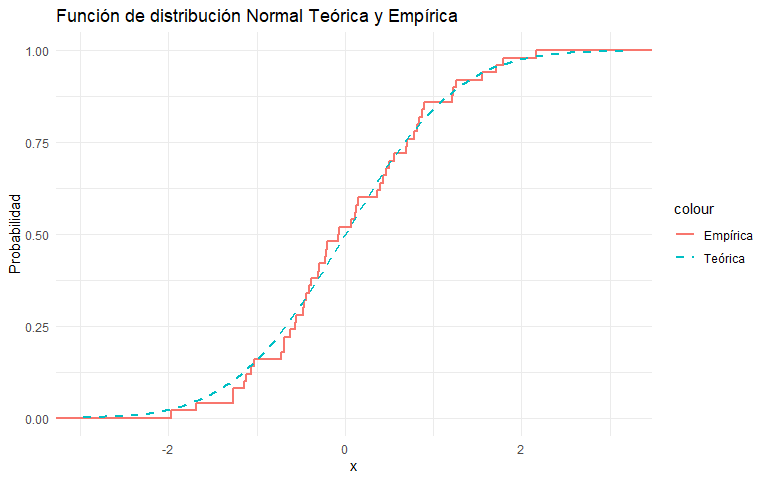
\includegraphics[width=\textwidth]{assets/TeoricaEmpirica.png}
    \caption{Visualización de una distribución teórica y empírica}
    \label{fig:theorical_vs_empirical}
\end{figure}

\subsection{Test Chi-Cuadrado de Bondad de Ajuste}

Sea $X_1,\dots,X_n$ con distribución F discreta:
\[
    \begin{matrix}
        C_1 \to P_1\\
        \dots \\
        C_k \to P_k
    \end{matrix}
    \quad
    p_j \geq 0,
    \quad \sum_{j=1}^{n} p_j=1
\]
Caso en el que $F_0$ completamente especificada bajo $H_0$:
\[
    H_0: p=p^0 \quad p=(p_1,\dots,p_k)'
\]
\[
    H_1: p \neq p^0 \quad p^0=(p_1^0,\dots,p_k^0)'
\]
Este problema ya lo sabemos resolver: es un contraste para el parámetro p de una distribución multinomial.

Frecuencia observada en $C_j: f_j=\sum_{i=1}^{n} \mathbbm{1}_{(x_i=c_j)}, \quad j=1,\dots,k \quad \sum_{j=1}^{k} f_j=n$

Frecuencia esperada bajo $H_0$ en $C_j$:
\[
    e_j=n \cdot P_0(x=c_j)=n \cdot p_j^0
\]

\textbf{Ejemplo:}

Sea una variable aleatoria $X$ cuya función de masa de probabilidad es la siguiente
\[
    P(X = x) = 
    \left\{
        \begin{matrix}
            \frac{1}{3} & \text{si } x = 0 \\[0.5em]
            \frac{1}{3} & \text{si } x = 1 \\[0.5em]
            \frac{1}{3} & \text{si } x = 2
        \end{matrix}
    \right.
\]

Entonces la hipotesis nula para el test será que

\[
    H_0:\quad p_1=\frac{1}{3} \quad p_2=\frac{1}{3} \quad p_3=\frac{1}{3}
\]

Tomando una muestra de n=10 quedan 7 ceros, 2 unos y 1 dos.

\vspace{5mm}

A simple vista no parece que siga esa distribución. Usaremos un estadístico para medir que tan diferente es de nuestra distribución pues lo que esperabamos obtener es:
\[
    \begin{matrix}
        e_1=3,33\\
        e_2=3,33\\
        e_3=3,33
    \end{matrix}
\]
El test $\chi^2$ de ajuste proporciona unas bases probabilisticas para decidir si las diferencias son suficientemente grandes tal que no hayan ocurrido por puro azar. Se define como
\[
    \chi^2=\sum_{j=1}^{k} \frac{(f_j-e_j)^2}{e_j}
\]
Este estadístico es lo que se conoce como distancia $\chi^2$ entre $f_j$ y $e_j$. Para valores grandes en $\chi^2$ implica frecuencias observadas y esperadas muy diferentes. 

\vspace{5mm}

\noindent Fijado $\alpha$:
\begin{itemize}
    \item Región critica: ($\chi^2 > C_\alpha$)
    \item p-valor: $p_0(\chi^2>X_{obs})=p_0(\chi^2>t_{obs})$
\end{itemize}

Necesitamos conocer la distribución del estadístico bajo $H_0$.
Se podría conocer de forma exacta aunque es muy complejo, por ello, nos interesará la distribución asintótica para $n$ grande.

\smallskip

\noindent \textbf{Resultado:}
\[
    \lim_{n \to \infty} P_0(\chi^2 \leq Z)=P(\chi^2_{k-1} \leq Z)
\]
La distribución asintótica del estadístico $\chi^2$ bajo $H_0$ es $\chi^2_{k-1}$ $g'$.

Ya hemos visto que en este contexto $ F_0 $ es una distribución multinomial. 
Vamos a ver que el estadístico $ T $ bajo $ H_0 $ para el modelo multinomial con $ k-1 $ parámetros libres es asintóticamente equivalente al estadístico $ \chi^2_1 $.

\begin{proofs}
    Estadístico RV para:
    \[
        H_0: F = F_0
    \]
    \[
        H_1: F \neq F_0
    \]
    Recordemos:
    \[
        L(p, x) = \prod_{j=1}^{k} p_j^{f_j} \quad \implies \quad \log L(p, x) = \sum_{j=1}^{k} f_j \log p_j
    \]
    El estadístico es:
    \[
        T = 2 \left[\log L(\widehat{p}, x) - \log L(p_0, x)\right] = 2 \left[ \sum_{j=1}^{k} f_j \log \widehat{p_j} - \sum_{j=1}^{k} f_j \log p_j^0 \right] 
    \]
    \[
        = -2 \sum_{j=1}^{k} \left( \log p_j^0 - \log \widehat{p_j} \right)
    \]
    Aproximamos $\log p_j^0$ por un desarrollo de Taylor en torno a $\log \widehat{p_j}$:
    \[
        \log p_j^0 \approx \log \widehat{p_j} + (p_j^0 - \widehat{p_j}) \frac{1}{\widehat{p_j}} - \frac{(p_j^0 - \widehat{p_j})^2}{2 \cdot \widehat{p_j}^2}+ \dots
    \]
    \[
        \to \log p_j^0- \log \widehat{p_j}\thickapprox (p^0_j-\widehat{p_j}) \frac{1}{\widehat{p_j}}- \frac{(p^0_j-\widehat{p_j})^2}{2}\frac{1}{\widehat{p_j^2}}
    \]
\end{proofs}

\newpage

\begin{proofs*}
    Sabiendo que $\widehat{p_j}=\frac{f_j}{n}$
    \[
        =\left(p_j^0-\frac{f_j}{n}\right) \cdot \frac{n}{f_j} - \frac{\left(p_j^0-\frac{f_j}{n}\right)^2}{2}\cdot \left(\frac{n}{f_j}\right)^2 \xrightarrow{c.s.} 0
    \]
    Esto converge a 0, ya que, por la Ley de los Grandes Números (LGN), $\frac{F_j}{n}$ es un estimador consistente de $p_j$:
    \[
        \lim_{n \to \infty} P \left( \left| \frac{F_j}{n} - p_j \right| > \varepsilon \right) = 0 \quad \forall \varepsilon>0
    \]
    Por lo tanto, el estadístico T queda:
    \[
        T = -2 \sum_{j=1}^{k} \left( n \cdot p_j^0 - f_j \right) + \frac{\sum_{j=1}^{k} (f_j - n \cdot p_j^0)^2}{f_j}
    \]
\end{proofs*}

El text $\chi^2$ y el TRV son asintóticamente equivalentes y como TRV converge a $\chi^2_{k-1}$, el estadístico $\chi^2$ también.
Fijado un $\alpha$.
\begin{itemize}
    \item Región critica: $P_0(\chi^2 \geq C_\alpha) \quad C_\alpha=qchisq(1-\alpha,k-1)$
    \item p-valor: $P_0(\chi^2 \geq t_{obs})=1-qchisq(t_{obs},k-1)$
\end{itemize}

\noindent \textit{Nota}:

Esta aproximación es válida para frecuencias mayores o iguales a 5

\vspace{5mm}

\textbf{Ejercicio 1}: Script R

\vspace{5mm}

\textbf{Ejercicio 4}: En una fábrica con 220 empleados, el número de trabajadores que tuvieron accidentes se recoge en latabla siguiente:

\begin{table}[!h]
    \centering
    \begin{tabular}{|c|c|c|c|c|c|c|c|}
        \hline
        {Nº accidentes} & 0 & 1 & 2 & 3 & 4 & 5 & 6+ \\ \hline
        {Nº trabajadores} & 181 & 9 & 4 & 10 & 7 & 4 & 5 \\ \hline
    \end{tabular}
\end{table}

¿Son estos datos consistentes con la distribución de Poisson con $\lambda=1$?

Tenemos una hipótesis compuesta ya que no conocemos el parámetro de la Poisson.
Si nos dijeran $P(1)$ sería simple.

\[
    f(x,1)=\frac{e^{-1}\cdot \lambda^x}{x!}=\frac{e^{-1}}{x!}
\]
\[
    p_0^0=e^{-1} ,\quad p_1^0=e^{-1} ,\quad p_2^0=\frac{e^-1}{2} ,\quad \dots,\quad p_6^0=1-\sum_{j=0}^{b}p_j^0
\]

Calculamos las frecuencias esperadas

\[
    e_0=220 \cdot e^{-1},\quad e_1=220 \cdot e^{-1}, \quad \dots
\]
\[
    \chi^2=\frac{(181-220 \cdot e^{-1})^2}{220 \cdot e^{-1}}+\dots
\]

Por tanto concluimos que es muy probable que no siga una P(1)

\textbf{Ejercicio 10:} Se lanza una moneda hasta que aparece la primera cara. Este experimento se repite 100 veces. LAs frecuencias observadas del numero de ensayos necesarios hasta que aparece la primera cara son:

\begin{table}[!h]
    \centering
    \begin{tabular}{|c|c|c|c|c|c|}
        \hline
        {Nº ensayos} & 1 & 2 & 3 & 4 & 5+ \\ \hline
        {Frecuencia} & 40 & 32 & 15 & 7 & 6 \\ \hline
    \end{tabular}
\end{table}

¿Se puede concluir que la moneda es perfecta?

Distribución geométrica:
\[
    P_p(X=k)=(1-p)^{k-1}p \quad o \quad P_p(X=k)=(1-p)^{k}p
\]
Probabilidad bajo $H_0$.
\[
    p_1^0=\frac{1}{2} \quad p_2^0=\frac{1}{2^2} \quad \dots \quad p_5=1-\sum_{k=1}^{4} p_k
\]

Como $H_0$ es ``Los datos provienen de una distribución geométrica $\left(\frac{1}{2}\right)$''.

Según el test, no rechazamos $H_0$.

Si en realidad los datos vienen de una distribución geométrica $\left(\frac{1}{3}\right)$,  
¿cuál es la probabilidad de que el test lo detecte?  
¿Y si vienen de una distribución geométrica $(0.52)$?

\subsection{Distribución del test bajo $H_1$}

Podemos aumentar la potencia sacrificando $\alpha$ o aumentando el tamaño de la muestra.  
Si queremos asegurar una potencia de, por ejemplo, $0.8$ o $0.9$, necesitamos calcular cuánto debe valer $n$.

Para esto, necesitamos conocer la distribución del test bajo $H_1$.

Resultado:
\[
\lim_{n \to \infty} P_{\theta_1} (\chi^2_{k-1} \leq t) = P(\chi^2_{k-1}(\delta) \leq t)
\]
Donde $\delta$ es el parámetro de descentralidad para la $\chi^2_{k-1}$ descentrada.

\textit{\textbf{Definición:}} La distribución asintótica bajo $H_1$ del estadístico $\chi^2$ de prueba de ajuste es una $\chi^2$ descentrada con $k-1$ grados de libertad y parámetro de descentralidad $\delta$.

La demostración no está incluida en este curso. Sin embargo, hacemos algunos comentarios sobre esta definición:

\textbf{Comentarios:} %Los comentarios eran formulajos y no me compilan
\begin{enumerate}
    \item   \begin{itemize}
        \item Si $X$ es una variable aleatoria tal que $X \sim N(0,1)$, entonces $X^2 \sim \chi^2_1$.
        \item Si $X_1, \dots, X_n$ son v.a.i.i.d. $N(0,1)$, entonces $\sum_{i=1}^{n} X_i^2 \sim \chi^2_n$.
        \item Si $X_1, \dots, X_n$ son v.a.i.i.d. $N(\mu, \sigma^2)$, entonces 
        $
        \sum_{i=1}^{n} \left( \frac{X_i}{\sigma} \right)^2 \sim \chi^2_n
        $
        descentrada con parámetro $\delta$.
    \end{itemize}
    \item Para contrastar 
    \[
    \begin{matrix}
        H_0: p_0 = (p_1^0, \dots, p_k^0) \\
        H_1: p \neq p^0
    \end{matrix}
    \]
    si bajo $H_1$ la alternativa 
    es $p = (p_1^1, \dots, p_k^1)$, el test $\chi^2$ sigue 
    una distribución $\chi^2_{k-1}(\delta)$, donde $\delta$ 
    mide la distancia entre los dos vectores:
    \[
    \Delta = \sum_{j=1}^{k} \frac{(p_j^1 - p_j^0)^2}{p_j^0}; \quad \delta = n \cdot \Delta
    \]
    O equivalentemente:
    \[
    \delta = \sum_{j=1}^{k} \frac{\left( n \cdot p_j^1 - n \cdot p_j^0 \right)^2}{n \cdot p_j^0}.
    \]
    \item Existen tablas para $\chi_{k-1}^{2'}(\delta)$ (por ejemplo, las tablas estándar de $\chi^2$ descentrada).
\end{enumerate}

\subsubsection*{Ejercicio 11:}  
Durante 60 meses consecutivos se observó la variable aleatoria X="nº de accidentes al mes en un cruce de carreteras". Los resultados fueron:

\begin{table}[!h]
    \centering
    \begin{tabular}{|c|c|c|c|c|}
        \hline
        {$X$} & 0 & 1 & 2 & 3+ \\ \hline
        {Nº de meses} & 23 & 18 & 12 & 7 \\ \hline
    \end{tabular}
\end{table}

\begin{enumerate}[label=\alph*)]
    \item Contrastar la hipótesis de que la distribución de X es geométrica:
    \[
        G(\theta);p_\theta(X=x)=\theta \cdot (1- \theta)^x, \quad X=0,1,2,\dots
    \]

    $H_0: X \sim G(\theta)=$EMV para $X \in \{0,1,2,3+\}$

    \[
        P_0^0=\theta, \quad P_1^0=\theta \cdot (1-\theta), \quad P_2^0=\theta \cdot (1-\theta)^2, \quad P_3^0=(1-\theta)^3
    \]
    \[
        L(\theta,f)=\prod_{j=1}^{4}[p_j^0]^{f_i}= \theta^{23}\cdot(\theta \cdot (1-\theta))^18 \cdot (\theta \cdot (1-\theta)^2)^12 \cdot ((1-\theta)^3)^7
    \]
    \[
        log L(\theta,f)=53 \log \theta+63 \log (1-\theta)
    \]
    \[
        \frac{d \log(\theta,f)}{d \theta}=\frac{53}{\theta}-\frac{63}{1-\theta} \Longrightarrow \widehat{\theta}=\frac{53}{53+63}
    \]
    Test $\chi^2$:
    \[
        \widehat{\chi^2}=\sum_{j=0}^{3} \frac{(f_j-60\cdot P_l^0(\widehat{\theta}))^2}{60 \cdot p_j^0(\widehat{\theta})} \sim \chi^2_2
    \]

    \item Potencia de $H_0:G(0.4) \quad B_n(2,0.6)$:
    \[
        P_1(\chi^2> C_{0.05})=P(\chi_3^2(\delta)>C_{0.05})
    \]
    \[
        S=n \cdot \Delta, \quad \Delta=\sum_{j=0}^{3} \left(\frac{(p_j^0-p_j^1)^2}{p_j^0}\right)
    \]
\end{enumerate}
